\documentclass[11pt,a4paper]{article}
\usepackage[utf8]{inputenc}
\usepackage[T1]{fontenc}
\usepackage{textcomp}
\usepackage{amssymb,adjustbox}
\usepackage{booktabs,graphicx,geometry,float,caption,xcolor,array,amsmath}
\usepackage[hidelinks]{hyperref}
\geometry{margin=2.3cm}
\captionsetup{font=small,labelfont=bf}
\setlength{\parskip}{0.45em}
\setlength{\parindent}{0pt}
\renewcommand{\arraystretch}{1.12}
\newcommand{\tp}[1]{\texttt{#1}}
\renewcommand{\tablename}{Tabela}
\renewcommand{\figurename}{Figura}
\sloppy\hyphenpenalty=10000\tolerance=3000\emergencystretch=4em
\renewcommand{\today}{Novembro de 2026}

\title{\textbf{Trabalho Prático III -- Introdução a Bancos de Dados}\\[0.3em]
\large Armazenamento, índices, otimizador de consultas e transações no PostgreSQL}
\author{Ruthelene Rodrigues Farias\\Matrícula 22552011\\UFAM / IComp -- 2026/02}
\date{Novembro de 2026}

\begin{document}
\maketitle

\section*{Visão geral}
Todos os resultados deste relatório foram produzidos pelos programas do repositório (\tp{src/t01\_sistema.py} a \tp{src/t17\_reservas.py}), executados por \tp{make parteI}, \tp{parteII}, \tp{parteIII} e \tp{parteIV} sobre PostgreSQL 16 em contêiner Docker, no GitHub Codespaces. Cada programa grava um arquivo JSON em \tp{resultados/}, e as tabelas da Seção 9.3 foram extraídas desses arquivos. Os parâmetros individuais, calculados a partir da matrícula, estão na Tabela~\ref{tab:params}.

\begin{table}[H]\centering\small
\caption{Parâmetros individuais (\texttt{params.json}).}\label{tab:params}
\begin{adjustbox}{max width=\linewidth}\begin{tabular}{ll}
\toprule
Parâmetro & Valor \\
\midrule
Matrícula & 22552011 \\
Fator de escala TPC-H (\texttt{sf}) & 0,1 \\
Consultas TPC-H & 1, 3, 5, 11, 14, 19, 20, 21 \\
\texttt{qgen\_seed} & 567059 \\
\texttt{t\_seed} & -0,980958 \\
Valores distintos de \texttt{v} & 100 \\
\texttt{fillfactor} & 70, 85, 95, 100 \\
Filme-alvo (T14) & American Beauty \\
Votos baixo / alto (T12, T16) & 1.000 / 35.000 \\
Letras de prefixo / sufixo (T15) & C / I \\
Assentos / espera de escolha (T17) & 120 / 0,1 s \\
Agentes \texttt{k} & 1, 2, 4, 6, 8, 10 \\
\bottomrule
\end{tabular}\end{adjustbox}
\end{table}

%%% ------------------------------------------------------------------
\section*{9.1 Decisões de projeto}
\textbf{Organização.} Cada tarefa é um programa independente que lê \tp{params.json}, executa o experimento e grava seu JSON por uma função comum. As partes são executadas em ordem pelo \tp{Makefile}, e o verificador (\tp{make test}) refaz medições de forma independente e compara com o que foi registrado. Na última execução anterior à inclusão deste relatório, todas as verificações dos resultados passaram (156 de 157; a restante era a presença deste PDF).

\textbf{Parte I.} Na T2 foi criado um arquivo temporário de 256 MiB, lido em blocos de 8 KiB com \tp{O\_DIRECT} (contorna o cache de páginas do sistema operacional): uma passada sequencial sobre os 32.768 blocos e 20.000 leituras em posições sorteadas (semente fixa). A razão é o tempo por bloco aleatório dividido pelo tempo por bloco sequencial. Na T4 cada consulta foi executada uma única vez com \tp{EXPLAIN (ANALYZE, BUFFERS)}; portanto, os blocos ``read'' refletem execução com cache parcialmente frio. O ``acesso dominante'' é uma heurística: a varredura que processa mais linhas no plano; o plano completo está em \tp{resultados/t04.json}.

\textbf{Parte II.} A tabela \tp{t} é criada com a função do template (semente individual). Os índices foram criados com \tp{max\_parallel\_maintenance\_workers = 0}. A consulta medida é a igualdade \tp{v = 50} (metade de $C = 100$). Na T7 o paralelismo de consulta foi desligado, os contadores de \tp{t} foram zerados com \tp{pg\_stat\_reset\_single\_table\_counters} e o \emph{flush} das estatísticas foi forçado antes de ler \tp{pg\_statio\_user\_tables}; a mesma execução fornece os blocos de \tp{EXPLAIN (BUFFERS)}. O mesmo código serve a T9 e a T10, que só diferem pela ordem do índice (\tp{v DESC NULLS FIRST}) e pela lista de \emph{fillfactors}.

\textbf{Parte III.} Consultas de T12: seletiva \tp{votes > 35000} e não seletiva \tp{votes > 1000}. O limiar foi procurado com \tp{EXPLAIN} (sem executar) para \tp{votes < X}, com $X$ crescendo de 50 em 50, até o primeiro plano \tp{Seq Scan}. Em T11, o número de chaves por folha vem de \tp{bt\_page\_stats}; os blocos de dados por chave são medidos pelo \tp{ctid}; já os blocos-folha por chave são uma \emph{estimativa} ($\max(1, \text{folhas}/\text{chaves distintas})$). Na T15 os índices criados são \tp{title text\_pattern\_ops}, \tp{substr(title,1,1)} e \tp{reverse(title) text\_pattern\_ops}, seguidos de \tp{ANALYZE} (necessário para haver estatísticas das expressões); o programa também registra o plano com \tp{enable\_seqscan = off} para mostrar se o índice seria possível. Na T16 o \tp{STATISTICS} de \tp{votes} é restaurado ao padrão no final.

\textbf{Parte IV: reservas.} A tabela é \tp{assentos(num\_voo, disp)}, em que \tp{num\_voo} identifica cada um dos 120 assentos (o enunciado fixa duas colunas, então a coluna \tp{num\_voo} faz o papel de identificador do assento). O passo 3 é \tp{UPDATE assentos SET disp = false WHERE num\_voo = X AND disp = true}. \emph{A garantia de que nenhum assento é reservado duas vezes vem dessa condição, e não do nível de isolamento.} O conflito é detectado de três formas: (i) o \tp{UPDATE} não altera linha (o assento já foi tomado); (ii) falha de serialização (SQLSTATE 40001); (iii) \emph{deadlock} (40P01). Nos três casos faz-se \tp{ROLLBACK} e uma nova tentativa completa (novo passo 1, nova escolha aleatória), e o número de tentativas de cada cliente é registrado. Cada agente é uma \emph{thread} com sua própria conexão; os 120 clientes ficam numa fila compartilhada; o relógio só inicia quando todos os agentes estão conectados (barreira) e termina quando o último cliente é atendido. As reservas são gravadas em \tp{reservas\_log} depois da medição, e o programa aborta se houver assento repetido, cliente sem reserva ou número de assentos ocupados diferente de 120. Na versão \emph{a} os três passos formam uma só transação; na versão \emph{b}, o passo 1 é uma transação, a espera de 0,1 s ocorre fora de transação, e o passo 3 é outra transação.

%%% ------------------------------------------------------------------
\section*{9.2 Previsão antes da medição}
As previsões foram escritas em \tp{docs/previsao.md} e commitadas antes de qualquer arquivo de \tp{resultados/} (commit \tp{0cde786}; o commit \tp{4f1310a} apenas removeu uma linha residual de formatação, sem mudar as previsões). O verificador confirma a ordem (``previsao.md versionado antes de resultados/''). Resumo do que foi previsto:

\begin{table}[H]\centering\small
\caption{Resumo das previsões registradas.}\label{tab:prev}
\begin{adjustbox}{max width=\linewidth}\begin{tabular}{lp{11cm}}
\toprule
Item & Previsão \\
\midrule
Páginas de \tp{t} & 443 páginas, 226 tuplas por página (36 B por tupla com ponteiro; 8168 B úteis por página) \\
Altura do índice & 1 para 100.000 tuplas (cerca de 90 páginas); 2 para 1.000.000 (850--900 folhas), graças à deduplicação ($C=100$) \\
\emph{Fillfactor} & tamanho 70 $>$ 85 $>$ 95 $>$ 100; altura igual; consulta praticamente igual; criação um pouco mais lenta com \emph{fillfactor} baixo; índice descendente igual ao crescente \\
T12 & seletiva: Index/Bitmap Scan; não seletiva: Seq Scan; limiar entre 5\% e 20\% das linhas \\
T15 & \tp{LIKE 'C\%'}, \tp{substr} e \tp{reverse} passam a usar índice; \tp{LIKE '\%I'} continua em Seq Scan \\
T16 & erro pequeno em \tp{votes < 1000}; erro relativo maior em \tp{votes > 35000}; \tp{STATISTICS 1000} aproxima da realidade \\
T17 & a/RC: cai com $k$, menos que $1/k$; a/SERIALIZABLE: pouca melhora ou piora; b/RC: quase $1/k$; b/SERIALIZABLE: perto de b/RC, um pouco acima; b mais rápida que a \\
\bottomrule
\end{tabular}\end{adjustbox}
\end{table}

%%% ------------------------------------------------------------------
\section*{9.3 Medição}
\subsection*{Parte I}
\begin{table}[H]\centering\small
\caption{T1 -- identificação do sistema (ambiente do GitHub Codespaces).}\label{tab:t1}
\begin{adjustbox}{max width=\linewidth}\begin{tabular}{lp{9cm}}
\toprule
Item & Valor \\
\midrule
CPU & AMD EPYC 7763 64-Core Processor (2 núcleos visíveis) \\
Memória RAM & 7.942 MB \\
Disco (capacidade do sistema de arquivos) & 33,6 GB \\
Caches & L1d 32 KiB; L1i 32 KiB; L2 512 KiB; L3 32 MiB \\
Sistema operacional / kernel & Debian GNU/Linux 13 (trixie) / 6.8.0-1064-azure \\
PostgreSQL & 16.15 \\
\texttt{block\_size} & 8192 B \\
\texttt{shared\_buffers} / \texttt{effective\_cache\_size} & 128MB / 4GB \\
\texttt{seq\_page\_cost} / \texttt{random\_page\_cost} & 1 / 4 \\
\texttt{work\_mem} / \texttt{default\_statistics\_target} & 4MB / 100 \\
\bottomrule
\end{tabular}\end{adjustbox}
\end{table}
\begin{table}[H]\centering\small
\caption{T2 -- armazenamento.}\label{tab:t2}
\begin{adjustbox}{max width=\linewidth}\begin{tabular}{lp{9cm}}
\toprule
Item & Valor \\
\midrule
Bloco do sistema de arquivos (\texttt{stat -f} / \texttt{stat}) & 4096 B / 4096 B \\
Bloco do PostgreSQL & 8192 B \\
Modo de leitura / arquivo de teste & O\_DIRECT / 256 MiB \\
Leitura sequencial & 32.768 blocos de 8 KiB: 41,5 \textmu s/bloco (188,4 MiB/s) \\
Leitura aleatória & 20.000 blocos: 35,2 \textmu s/bloco (28.422 IOPS) \\
Razão custo aleatório / sequencial & 0,85 \\
\bottomrule
\end{tabular}\end{adjustbox}
\end{table}
\begin{table}[H]\centering\small
\caption{T3 -- TPC-H carregado com \texttt{sf} = 0,1.}\label{tab:t3}
\begin{adjustbox}{max width=\linewidth}\begin{tabular}{lrrr}
\toprule
Tabela & Linhas & Tabela (MiB) & Total com índices (MiB) \\
\midrule
\texttt{region} & 5 & 0,01 & 0,02 \\
\texttt{nation} & 25 & 0,01 & 0,04 \\
\texttt{part} & 20.000 & 3,25 & 3,73 \\
\texttt{supplier} & 1.000 & 0,34 & 0,43 \\
\texttt{partsupp} & 80.000 & 13,69 & 16,95 \\
\texttt{customer} & 15.000 & 2,82 & 3,31 \\
\texttt{orders} & 150.000 & 20,69 & 25,18 \\
\texttt{lineitem} & 600.572 & 88,19 & 114,41 \\
\bottomrule
\end{tabular}\end{adjustbox}
\end{table}
\begin{table}[H]\centering\small
\caption{T4 -- consultas TPC-H com \texttt{EXPLAIN (ANALYZE, BUFFERS)} (uma execução de cada).}\label{tab:t4}
\begin{adjustbox}{max width=\linewidth}\begin{tabular}{llp{3.3cm}rrrr}
\toprule
Consulta & Acesso dominante & Junções & Custo est. & Linhas est./reais & Blocos hit/read & Tempo (ms) \\
\midrule
q01 & Seq Scan em lineitem & -- & 24.014,63 & 6 / 4 & 2.372 / 8.930 & 658,4 \\
q03 & Seq Scan em orders & Hash Join, Nested Loop & 22.478,73 & 31.680 / 1.164 & 53.105 / 8.772 & 189,1 \\
q05 & Seq Scan em orders & Hash Join, Nested Loop & 12.817,73 & 25 / 5 & 23.056 / 850 & 49,4 \\
q11 & Index Scan em partsupp & Nested Loop & 1.045,77 & 1.067 / 18 & 8.698 / 40 & 15,3 \\
q14 & Seq Scan em part & Hash Join & 16.979,21 & 1 / 1 & 10.596 / 2.062 & 95,9 \\
q19 & Seq Scan em part & Nested Loop & 7.066,14 & 1 / 1 & 1.656 / 289 & 14,5 \\
q20 & Index Scan em lineitem & Hash Join, Nested Loop & 8.853,21 & 11 / 20 & 9.226 / 1.537 & 26,8 \\
q21 & Seq Scan em lineitem & Hash Join, Nested Loop & 18.189,44 & 1 / 34 & 67.308 / 3.315 & 183,5 \\
\bottomrule
\end{tabular}\end{adjustbox}
\end{table}

\subsection*{Parte II}
\begin{table}[H]\centering\small
\caption{T5, T6 e T7 -- tabela \texttt{t} (100.000 tuplas).}\label{tab:t567}
\begin{adjustbox}{max width=\linewidth}\begin{tabular}{lp{9.2cm}}
\toprule
Item & Valor \\
\midrule
T5 -- soma de \texttt{v} / tuplas & 4.955.172 / 100.000 \\
T6 -- \texttt{relpages} / \texttt{reltuples} & 443 / 100.000 \\
T6 -- bytes / \texttt{block\_size} = páginas & 3.629.056 / 8192 = 443 \\
T6 -- tuplas por página (média) & 225,73 \\
T7 -- \texttt{pg\_stats} de \texttt{k} & n\_distinct = -1; correlação = 1,00; histograma com 100 faixas \\
T7 -- \texttt{pg\_stats} de \texttt{v} & n\_distinct = 100; correlação = 0,006; 100 valores comuns (freq. entre 0,85\% e 1,15\%); sem histograma \\
T7 -- consulta \texttt{v = 50} (sem índice) & Seq Scan; 443 blocos em memória e 0 lidos (pg\_statio); EXPLAIN: 443 / 0 \\
\bottomrule
\end{tabular}\end{adjustbox}
\end{table}
\begin{table}[H]\centering\small
\caption{T8, T9 e T10 -- índice B-tree sobre \texttt{v} (consulta \texttt{v = 50}).}\label{tab:t8910}
\begin{adjustbox}{max width=\linewidth}\begin{tabular}{llrrrrrrl}
\toprule
Tarefa & Configuração & Págs. & Alt. & Folhas & Dens. (\%) & Criação (ms) & Consulta (ms) & Plano \\
\midrule
T8 (cresc.) & 100.000 tuplas, ff 90 (padrão) & 90 & 1 & 88 & 86,29 & 66 & 0,41 & Bitmap Heap Scan \\
T8 (cresc.) & 1.000.000 tuplas, ff 90 (padrão) & 854 & 2 & 847 & 89,50 & 999 & 4,55 & Bitmap Heap Scan \\
T9 (cresc.) & 1.000.000, ff 70 & 1084 & 2 & 1076 & 70,54 & 1.206 & 5,04 & Bitmap Heap Scan \\
T9 (cresc.) & 1.000.000, ff 85 & 854 & 2 & 847 & 89,50 & 1.064 & 4,49 & Bitmap Heap Scan \\
T9 (cresc.) & 1.000.000, ff 95 & 854 & 2 & 847 & 89,50 & 1.290 & 5,26 & Bitmap Heap Scan \\
T9 (cresc.) & 1.000.000, ff 100 & 854 & 2 & 847 & 89,50 & 892 & 4,35 & Bitmap Heap Scan \\
T10 (desc.) & 1.000.000, ff 100 & 854 & 2 & 847 & 89,50 & 943 & 4,82 & Bitmap Heap Scan \\
T10 (desc.) & 1.000.000, ff 70 & 1084 & 2 & 1076 & 70,54 & 1.211 & 7,13 & Bitmap Heap Scan \\
T10 (desc.) & 1.000.000, ff 85 & 854 & 2 & 847 & 89,50 & 883 & 6,41 & Bitmap Heap Scan \\
T10 (desc.) & 1.000.000, ff 95 & 854 & 2 & 847 & 89,50 & 1.012 & 6,14 & Bitmap Heap Scan \\
T10 (desc.) & 1.000.000, ff 100 & 854 & 2 & 847 & 89,50 & 1.261 & 6,20 & Bitmap Heap Scan \\
\bottomrule
\end{tabular}\end{adjustbox}
\end{table}

\subsection*{Parte III}
\begin{table}[H]\centering\small
\caption{T11 -- índices de \texttt{movie} (1.844 linhas em 15 blocos).}\label{tab:t11}
\begin{adjustbox}{max width=\linewidth}\begin{tabular}{llrrrrrr}
\toprule
Índice & Atributo & Alt. & Folhas & Chaves/folha (máx./média) & Distintas & Linhas/chave & Blocos de dados/chave \\
\midrule
\texttt{movie\_key} & \texttt{id} & 1 & 5 & 380 / 369,6 & 1.844 & 1,000 & 1,000 \\
\texttt{movie\_title} & \texttt{title} & 1 & 10 & 238 / 185,0 & 1.833 & 1,006 & 1,005 \\
\texttt{movie\_votes} & \texttt{votes} & 1 & 9 & 214 / 169,2 & 1.481 & 1,245 & 1,003 \\
\bottomrule
\end{tabular}\end{adjustbox}
\end{table}
\begin{table}[H]\centering\small
\caption{T12 -- consultas por intervalo. Limiar: \texttt{votes < X} passa a usar Seq Scan em X = 1.550 (677 linhas, 36,7\% da tabela).}\label{tab:t12}
\begin{adjustbox}{max width=\linewidth}\begin{tabular}{lrllrr}
\toprule
Consulta & Linhas & Plano & Custo & Blocos (hit) & Tempo (ms) \\
\midrule
Seletiva: \texttt{votes > 35000} & 6 & Index Scan & 8,49 & 3 & 0,015 \\
Não seletiva: \texttt{votes > 1000} & 1.516 (82,2\%) & Seq Scan & 38,05 & 15 & 0,353 \\
\bottomrule
\end{tabular}\end{adjustbox}
\end{table}
\begin{table}[H]\centering\small
\caption{T13 e T14 -- consultas equivalentes (T13: resultado = título devolvido; T14: American Beauty).}\label{tab:t1314}
\begin{adjustbox}{max width=\linewidth}\begin{tabular}{lllrr}
\toprule
Consulta & Linhas & Nós do plano & Custo & Tempo (ms) \\
\midrule
T13 -- \texttt{MAX} & Star Wars & Index Scan, Result, Limit, Index Only Scan & 35,37 & 0,110 \\
T13 -- \texttt{>= ALL} & Star Wars & Seq Scan, Materialize, Seq Scan & 43.620,99 & 1,239 \\
T14 -- subconsulta & 9 & Index Scan, Index Scan & 43,34 & 0,096 \\
T14 -- auto-junção & 9 & Nested Loop, Index Scan, Index Scan & 49,49 & 0,025 \\
\bottomrule
\end{tabular}\end{adjustbox}
\end{table}
\begin{table}[H]\centering\small
\caption{T15 -- planos antes e depois de criar os índices \texttt{text\_pattern\_ops}, sobre \texttt{substr} e sobre \texttt{reverse}.}\label{tab:t15}
\begin{adjustbox}{max width=\linewidth}\begin{tabular}{lrp{4.2cm}p{4.2cm}}
\toprule
Consulta & Linhas & Antes (custo) & Depois (custo) \\
\midrule
\texttt{prefixo\_like} & 130 & Seq Scan (38,05) & Bitmap Heap Scan, Bitmap Index Scan (22,19) \\
\texttt{prefixo\_substr} & 130 & Seq Scan (42,66) & Bitmap Heap Scan, Bitmap Index Scan (22,23) \\
\texttt{sufixo\_like} & 26 & Seq Scan (38,05) & Seq Scan (38,05) \\
\texttt{sufixo\_reverse} & 26 & Seq Scan (42,66) & Bitmap Heap Scan, Bitmap Index Scan (20,53) \\
\bottomrule
\end{tabular}\end{adjustbox}
\end{table}
\begin{table}[H]\centering\small
\caption{T16 -- estimativa de seletividade sobre \texttt{movie.votes}.}\label{tab:t16}
\begin{adjustbox}{max width=\linewidth}\begin{tabular}{lrrr}
\toprule
Consulta & Linhas reais & Estimadas (padrão, 100 faixas) & Estimadas (STATISTICS 1000) \\
\midrule
\texttt{votes < 1000} & 326 & 328 & 325 \\
\texttt{votes > 35000} & 6 & 12 & 5 \\
\bottomrule
\end{tabular}\end{adjustbox}
\end{table}

\subsection*{Parte IV}
\begin{table}[H]\centering\small
\caption{T17 -- reservas (120 assentos, 120 clientes). Speedup = tempo com $k=1$ dividido pelo tempo com $k$ agentes.}\label{tab:t17}
\begin{adjustbox}{max width=\linewidth}\begin{tabular}{llrrrrrrrrr}
\toprule
Ver. & Isolamento & $k$ & Tempo (s) & Speedup & Tent. média & Tent. máx. & Tent. total & Assento tomado & Falha 40001 & Deadlock \\
\midrule
a & read committed & 1 & 12,28 & 1,00 & 1,00 & 1 & 120 & 0 & 0 & 0 \\
a & read committed & 2 & 6,36 & 1,93 & 1,02 & 2 & 123 & 3 & 0 & 0 \\
a & read committed & 4 & 3,50 & 3,51 & 1,10 & 3 & 132 & 12 & 0 & 0 \\
a & read committed & 6 & 2,47 & 4,97 & 1,11 & 4 & 133 & 13 & 0 & 0 \\
a & read committed & 8 & 2,05 & 5,99 & 1,21 & 5 & 145 & 25 & 0 & 0 \\
a & read committed & 10 & 1,65 & 7,44 & 1,22 & 3 & 146 & 26 & 0 & 0 \\
a & serializable & 1 & 12,26 & 1,00 & 1,00 & 1 & 120 & 0 & 0 & 0 \\
a & serializable & 2 & 12,28 & 1,00 & 2,00 & 120 & 240 & 0 & 120 & 0 \\
a & serializable & 4 & 12,42 & 0,99 & 3,98 & 118 & 478 & 0 & 358 & 0 \\
a & serializable & 6 & 12,46 & 0,98 & 5,93 & 119 & 712 & 0 & 592 & 0 \\
a & serializable & 8 & 12,51 & 0,98 & 7,87 & 121 & 944 & 0 & 824 & 0 \\
a & serializable & 10 & 12,62 & 0,97 & 9,82 & 124 & 1.178 & 0 & 1058 & 0 \\
b & read committed & 1 & 12,33 & 1,00 & 1,00 & 1 & 120 & 0 & 0 & 0 \\
b & read committed & 2 & 6,38 & 1,93 & 1,02 & 2 & 123 & 3 & 0 & 0 \\
b & read committed & 4 & 3,50 & 3,52 & 1,10 & 4 & 132 & 12 & 0 & 0 \\
b & read committed & 6 & 2,58 & 4,78 & 1,18 & 3 & 141 & 21 & 0 & 0 \\
b & read committed & 8 & 1,96 & 6,28 & 1,18 & 3 & 142 & 22 & 0 & 0 \\
b & read committed & 10 & 1,69 & 7,29 & 1,18 & 4 & 141 & 21 & 0 & 0 \\
b & serializable & 1 & 12,31 & 1,00 & 1,00 & 1 & 120 & 0 & 0 & 0 \\
b & serializable & 2 & 8,21 & 1,50 & 1,32 & 4 & 158 & 4 & 34 & 0 \\
b & serializable & 4 & 5,65 & 2,18 & 1,79 & 8 & 215 & 10 & 85 & 0 \\
b & serializable & 6 & 3,49 & 3,53 & 1,57 & 6 & 189 & 16 & 53 & 0 \\
b & serializable & 8 & 2,98 & 4,13 & 1,82 & 10 & 218 & 19 & 79 & 0 \\
b & serializable & 10 & 3,42 & 3,60 & 2,46 & 11 & 295 & 22 & 153 & 0 \\
\bottomrule
\end{tabular}\end{adjustbox}
\end{table}

\begin{figure}[H]\centering
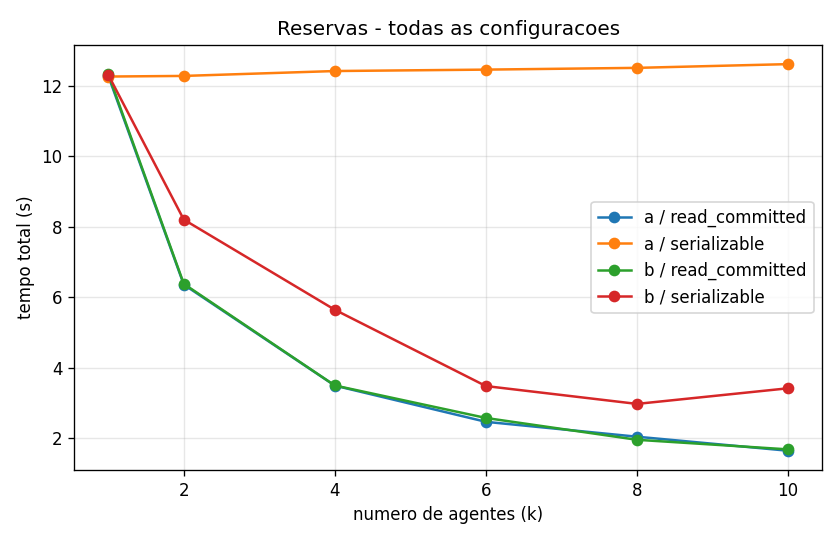
\includegraphics[width=0.78\textwidth]{../resultados/t18_comparativo.png}
\caption{T17 -- tempo total em função do número de agentes $k$, nas quatro configurações.}\label{fig:comp}
\end{figure}
\begin{figure}[H]\centering
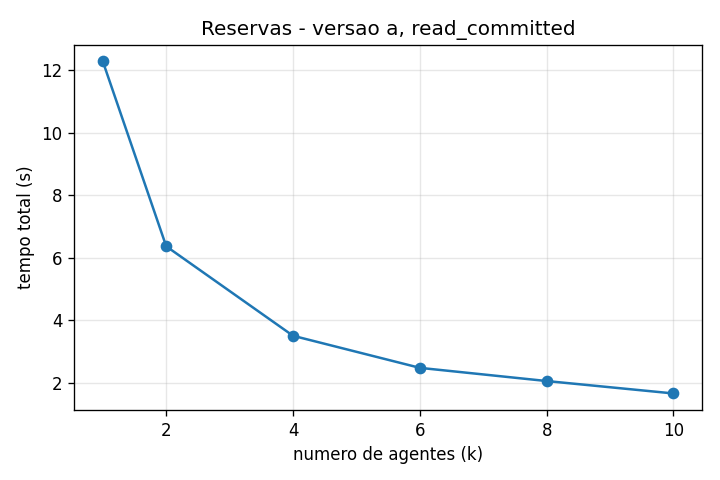
\includegraphics[width=0.48\textwidth]{../resultados/t18_a_read_committed.png}\hfill
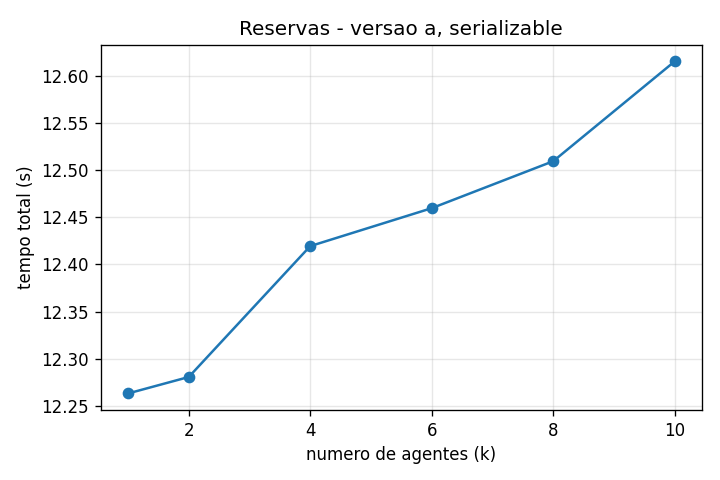
\includegraphics[width=0.48\textwidth]{../resultados/t18_a_serializable.png}\\[0.5em]
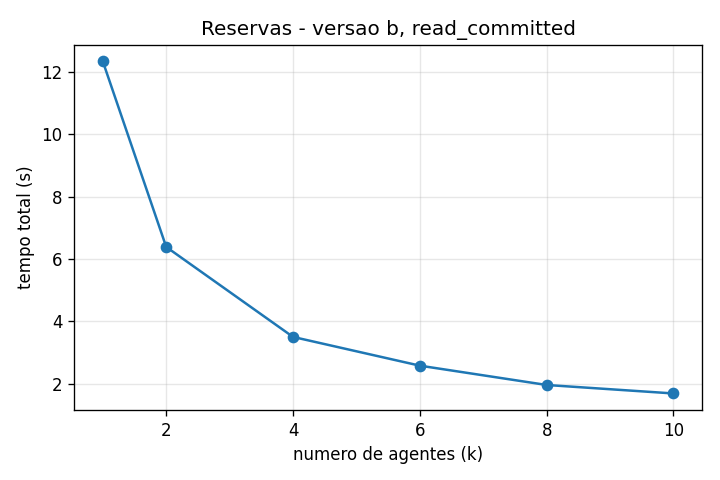
\includegraphics[width=0.48\textwidth]{../resultados/t18_b_read_committed.png}\hfill
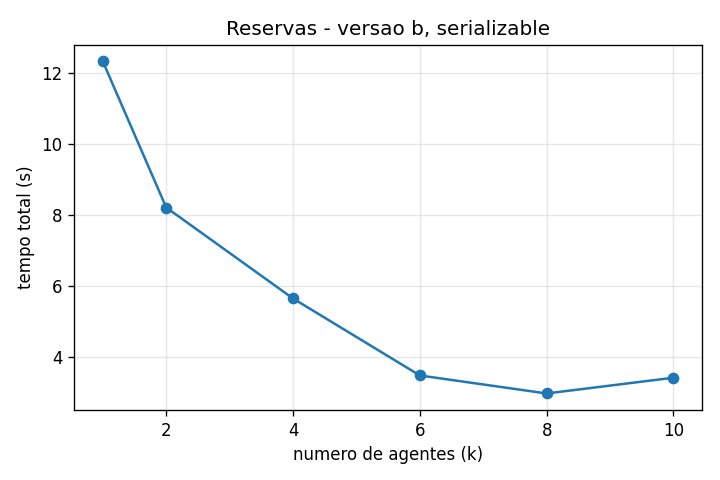
\includegraphics[width=0.48\textwidth]{../resultados/t18_b_serializable.png}
\caption{T17 -- gráficos individuais (versão a em cima, versão b embaixo; READ COMMITTED à esquerda, SERIALIZABLE à direita).}\label{fig:ind}
\end{figure}

%%% ------------------------------------------------------------------
\section*{9.4 Comparação e explicação das divergências}
\begin{table}[H]\centering\small
\caption{Previsto $\times$ medido.}\label{tab:comp}
\begin{adjustbox}{max width=\linewidth}\begin{tabular}{p{3.6cm}p{4.3cm}p{4.9cm}c}
\toprule
Item & Previsto & Medido & \\
\midrule
Páginas de \tp{t} & 443; 226 tuplas/pág. & 443; 225,73 (média) & \checkmark \\
Altura, 100.000 & 1 (cerca de 90 págs.) & 1 (90 págs., 88 folhas) & \checkmark \\
Altura, 1.000.000 & 2 (850--900 folhas) & 2 (847 folhas) & \checkmark \\
\emph{Fillfactor}: tamanho & 70 $>$ 85 $>$ 95 $>$ 100 & só o 70 difere (1084 págs.); 85, 95 e 100 = 854 & divergiu \\
\emph{Fillfactor}: criação & ligeiramente maior com \emph{ff} baixo & 883--1290 ms, sem tendência & inconclusivo \\
\emph{Fillfactor}: consulta & praticamente igual & 4,35--5,26 ms & \checkmark \\
Descendente & igual ao crescente & idêntico em páginas, folhas, altura & \checkmark \\
T12 seletiva / não seletiva & Index Scan / Seq Scan & Index Scan (6 linhas) / Seq Scan (82,2\%) & \checkmark \\
T12 limiar & 5\% a 20\% & 36,7\% ($X = 1550$) & divergiu \\
T15 & 3 passam a usar índice; sufixo não & exatamente isso (Bitmap Index Scan) & \checkmark \\
T16 & erro maior na cauda; mais estatística ajuda & 328 vs 326; 12 vs 6; com 1000: 325 e 5 & \checkmark \\
T17 a/RC & cai com $k$, menos que $1/k$ & 12,28 s $\to$ 1,65 s (speedup 7,4) & \checkmark \\
T17 a/SER & pouca melhora ou piora & constante, 12,3--12,6 s; tentativas $\approx k$ & \checkmark (mais extremo) \\
T17 b/RC & quase $1/k$ & 12,33 s $\to$ 1,69 s (speedup 7,3) & \checkmark \\
T17 b/SER & perto de b/RC & 3,42 s com $k=10$, o dobro de b/RC & divergiu \\
T17 a $\times$ b em RC & b mais rápida que a & praticamente iguais & divergiu \\
\bottomrule
\end{tabular}\end{adjustbox}
\end{table}

\subsection*{D1. \emph{Fillfactor}: só o valor 70 mudou o tamanho do índice}
Como $C = 100$, cada valor de \tp{v} aparece cerca de 10.000 vezes em 1.000.000 de tuplas, e o PostgreSQL 16 \emph{deduplica} entradas repetidas: guarda uma única tupla de índice com uma lista de ponteiros (6 B por ponteiro). Na construção do índice o tamanho dessa tupla é limitado a cerca de 10\% da página (algo como 800 B, aproximadamente 130 ponteiros). Assim, uma folha guarda poucas tuplas grandes, e o \emph{fillfactor} só pode mudar o conteúdo da folha em passos de uma dessas tuplas. A densidade medida é compatível com isso: 89,5\% corresponde a 9 tuplas por folha e 70,5\% a 7 tuplas. Com 9 tuplas $\times$ cerca de 130 ponteiros $\approx$ 1.200 ponteiros por folha, 1.000.000 de linhas ocupam algo entre 830 e 850 folhas, compatível com as 847 medidas. Os valores 85, 90 (padrão), 95 e 100 caem no mesmo número de tuplas por folha; só o 70 desce para 7, e então o índice cresce para 1076 folhas (cerca de 27\% a mais). Esta é uma \emph{hipótese coerente com os números}, não verificada diretamente (por exemplo, com \tp{pageinspect} ou criando o índice com \tp{deduplicate\_items = off}, caso em que se esperaria tamanho monotônico em relação ao \emph{fillfactor}).

\subsection*{D2. Tempos de criação e de consulta}
Cada configuração foi medida uma única vez. Os tempos de criação (883 a 1290 ms) variam sem relação monotônica com o \emph{fillfactor} (o 95 foi mais lento que o 70), então a diferença prevista, que é pequena, não é distinguível do ruído de uma medição única em máquina virtual compartilhada. Os tempos de consulta de T9 (4,35 a 5,26 ms) e de T10 (4,82 a 7,13 ms) também ficam na mesma faixa, e o plano é o mesmo em todos os casos.

\subsection*{D3. Limiar de T12 acima do previsto (36,7\% em vez de 5--20\%)}
A previsão supunha o comportamento de tabelas grandes, em que o acesso aleatório às páginas domina o custo do índice. A tabela \tp{movie} tem só 15 blocos. O custo do \tp{Seq Scan} é praticamente fixo: $15 \times 1 + 1.844 \times (0{,}01 + 0{,}0025) = 38{,}05$, exatamente o custo medido nas consultas T12 e T15. O plano por índice lê no máximo 15 blocos de dados (o número de blocos buscados satura), e seu custo cresce sobretudo com o número de linhas devolvidas (custos de CPU por tupla). Por isso o ponto de cruzamento só ocorre quando a consulta devolve uma fração grande da tabela. A previsão de 5--20\% valeria para uma tabela com milhares de páginas.

\subsection*{D4. Versões a e b praticamente iguais em READ COMMITTED}
Eu previ a versão b mais rápida. Em READ COMMITTED, uma transação só segura travas a partir do \tp{UPDATE} (a leitura do passo 1 não bloqueia ninguém), e a espera de 0,1 s da versão a acontece \emph{antes} do \tp{UPDATE}. Ou seja, nenhuma das duas versões segura travas durante a espera, e ambas leem a lista de assentos antes de esperar. Os conflitos vêm só de agentes que sorteiam o mesmo assento, o que ocorre com a mesma frequência nas duas.

\subsection*{D5. b/SERIALIZABLE bem acima de b/READ COMMITTED}
No nível SERIALIZABLE o PostgreSQL usa Serializable Snapshot Isolation (SSI), que aborta com 40001 quando detecta uma estrutura perigosa de dependências de leitura-escrita. Mesmo na versão b houve 34 a 153 falhas por configuração. Causas plausíveis (não separadas na medição): (i) quando dois agentes atualizam o mesmo assento, o SERIALIZABLE aborta o segundo com 40001, enquanto no READ COMMITTED o segundo reavalia a condição \tp{disp = true} e simplesmente conta como ``assento tomado''; (ii) as travas de predicado (SIREAD) da leitura de toda a tabela no passo 1 podem permanecer depois do \emph{commit}, enquanto houver transações concorrentes, e participar de conflitos com escritas posteriores. O tempo piorou de $k=8$ (2,98 s) para $k=10$ (3,42 s), junto com mais falhas (79 para 153), mas cada ponto é uma única execução e há variação entre execuções.

%%% ------------------------------------------------------------------
\section*{9.5 Análises por parte}
\subsection*{Parte I}
\textbf{Tipo de acesso e custo.} As consultas q01, q03, q05, q14, q19 e q21 têm uma varredura sequencial como acesso dominante, em geral com \emph{hash join}, e q11 e q20 têm acesso por índice com \emph{nested loop}. A q01 lê praticamente toda a \tp{lineitem} (11.302 blocos acessados, o número de páginas da tabela) e devolve só 4 grupos, daí o maior custo (24.014,63) e o maior tempo (658,4 ms). As consultas com filtros seletivos sobre dimensões pequenas (q11 e q20) usam índice e têm os custos mais baixos (1.045,8 e 8.853,2). A ordenação por custo e por tempo coincide em seis das oito posições (q01, q03, q21, q14, q05, q20); só q19 e q11, com tempos quase iguais (14,5 e 15,3 ms), trocam de lugar. O custo é uma unidade abstrata (1 = leitura sequencial de uma página), não milissegundos: o custo da q01 é cerca de 23 vezes o da q11, e o tempo, cerca de 43 vezes. As estimativas de linhas erram bastante: q03 estimou 31.680 linhas e devolveu 1.164; q11, 1.067 contra 18; q21, 1 contra 34. Como cada consulta foi executada uma vez, os blocos ``read'' mostram o efeito de cache frio (q01 leu 8.930 de 11.302 blocos fora do \tp{shared\_buffers}).

\textbf{Tamanho de bloco.} No PostgreSQL o bloco (8 KiB, medido em \tp{block\_size}) é definido na compilação (\tp{--with-blocksize}, de 1 a 32 KiB, potência de 2) e fixado quando o \emph{cluster} é criado com \tp{initdb}; para mudá-lo é preciso recompilar, criar um novo \emph{cluster} e recarregar os dados (\tp{pg\_dump}/restauração). No sistema de arquivos o bloco (4 KiB aqui, tanto em \tp{stat -f} quanto em \tp{stat}) é definido ao formatar a partição (por exemplo, \tp{mkfs}), e em Linux não pode exceder o tamanho da página de memória (4 KiB) para ser montado. Dentro de um contêiner o sistema de arquivos é o do hospedeiro, então o bloco não pode ser alterado de dentro do contêiner. Blocos maiores reduzem o número de operações em leituras sequenciais, mas desperdiçam leitura e escrita em acessos pontuais.

\textbf{Custo aleatório/sequencial medido.} Medimos razão 0,85 (35,2 \textmu s por bloco aleatório contra 41,5 \textmu s por bloco sequencial), enquanto o PostgreSQL assume \tp{random\_page\_cost}/\tp{seq\_page\_cost} = 4. Neste armazenamento (SSD virtualizado numa VM da Azure) não há penalidade de acesso aleatório; o valor 4 foi pensado para discos rotativos. Com razão próxima de 1, o planejador superestima o custo de acessos por índice e tende a preferir varreduras sequenciais mais cedo do que seria ideal; para SSD é comum usar valores perto de 1,1. A diferença de 15\% a favor do aleatório está dentro da variação esperada de uma única medição. A medição é limitada: uma \emph{thread}, \tp{O\_DIRECT} (sem \emph{readahead} do sistema operacional) e uma passada de cada tipo.

\subsection*{Parte II}
\textbf{\tp{relpages} e tuplas por página.} Cada tupla ocupa 24 B de cabeçalho (23 B arredondados) mais 8 B de dados (dois inteiros), ou seja, 32 B, mais 4 B do ponteiro de linha na página: 36 B. Descontados os 24 B do cabeçalho da página, sobram 8.168 B: $\lfloor 8168/36 \rfloor = 226$ tuplas por página. Então $\lceil 100.000/226 \rceil = 443$ páginas, valor medido em \tp{relpages} e em \tp{pg\_relation\_size} (3.629.056 B / 8192). A média de 225,73 é $100.000/443$: a última página fica incompleta.

\textbf{Estatísticas e acesso à tabela.} \tp{k} é único (\tp{n\_distinct = -1}) e totalmente correlacionado com a ordem física (correlação 1,0). \tp{v} tem 100 valores, cada um com frequência próxima de 1\%, e correlação 0,006 com a ordem física, isto é, as linhas de um mesmo valor estão espalhadas por toda a tabela. Como a lista de valores comuns já cobre todos os 100 valores, não há histograma. Com 226 tuplas por página e 1\% de linhas por valor, a fração de páginas com pelo menos uma linha com $v = 50$ é cerca de $1 - 0{,}99^{226} \approx 90\%$; por isso, sem índice, a consulta faz \tp{Seq Scan} (443 blocos, todos já em \tp{shared\_buffers}, porque 3,5 MB cabem nos 128 MB), e com índice o plano é \tp{Bitmap Heap Scan}: o índice não evita ler quase todas as páginas, e o \emph{bitmap} apenas as lê em ordem física. Os dois contadores (\tp{pg\_statio\_user\_tables} e \tp{EXPLAIN}) concordam: 443 blocos.

\textbf{Altura do índice.} Altura 1 significa que há um nível interno (a raiz) acima das folhas. Para 100.000 tuplas há 88 folhas e 90 páginas no total (metapágina + raiz + 88 folhas), então a raiz aponta diretamente para as folhas. Para 1.000.000 há 847 folhas e 854 páginas: descontadas a metapágina, sobram 6 páginas internas, a raiz e 5 intermediárias, cada uma com cerca de 170 ponteiros para folhas. As 847 folhas não cabem numa só página interna, então é preciso um nível a mais e a altura passa a 2. O número de folhas cresce quase linearmente (88 para 847, cerca de 9,6 vezes para 10 vezes mais tuplas), e a altura cresce com o logaritmo.

\textbf{\emph{Fillfactor}.} Tamanho: só o 70 aumenta o índice (1084 páginas contra 854, ver D1). Altura: 2 em todos. Tempo: a criação ficou entre 883 e 1290 ms e a consulta entre 4,35 e 5,26 ms, sem diferença atribuível ao \emph{fillfactor} numa execução única (ver D2). Um \emph{fillfactor} menor deixa espaço livre nas folhas para inserções futuras sem divisão de páginas, ao custo de um índice maior.

\textbf{Crescente e descendente.} O índice descendente (\tp{v DESC NULLS FIRST}) ficou idêntico em páginas, folhas, altura e densidade. Um índice B-tree pode ser percorrido nos dois sentidos, então para uma única coluna o sentido só importa em ordenações com colunas de direções mistas; como \tp{v} não tem NULL, \tp{NULLS FIRST} também não muda nada. O plano da igualdade foi o mesmo (\tp{Bitmap Heap Scan}); as diferenças de tempo (T10: 4,82 a 7,13 ms; T9: 4,35 a 5,26 ms) são de uma única medição.

\subsection*{Parte III}
\textbf{Por que o índice de \tp{votes} nem sempre é usado.} O planejador escolhe o plano de menor custo estimado. Para \tp{votes > 35000} (6 linhas) o índice custa 8,49 contra 38,05 do \tp{Seq Scan}; para \tp{votes > 1000} (82,2\% da tabela) a leitura sequencial compensa. O limiar medido foi $X = 1550$ (36,7\% das linhas), explicado em D3: numa tabela de 15 blocos, o índice só perde quando devolve uma fração grande das linhas.

\textbf{T13.} \tp{MAX(votes)} é reescrito pelo PostgreSQL como ``leia a última entrada do índice de \tp{votes}'' (\tp{Index Only Scan} com \tp{Limit 1}), executado uma vez; custo 35,37 e 0,11 ms. O \tp{>= ALL} não tem essa reescrita: cada uma das 1.844 linhas é comparada com os valores da subconsulta materializada, cerca de 3,4 milhões de comparações no pior caso; custo 43.620,99 (cerca de 1.200 vezes o do \tp{MAX}). O tempo real (1,24 ms, cerca de 11 vezes o do \tp{MAX}) é bem menor que a razão de custos, pois o \tp{>= ALL} para na primeira comparação que falha, o que o modelo de custo não prevê. Os dois devolvem o mesmo resultado.

\textbf{T14.} Subconsulta (custo 43,34) e auto-junção (49,49) devolvem as mesmas 9 linhas, mas os planos são diferentes: a subconsulta escalar é avaliada uma vez e vira constante para um \tp{Index Scan}; a junção usa \tp{Nested Loop} com dois \tp{Index Scan}. O planejador não transforma uma na outra porque não pode provar que o título é único: \tp{movie} tem 1.844 linhas e 1.833 títulos distintos (um título repetido faria a subconsulta falhar e a junção multiplicar linhas). Os tempos (0,096 ms e 0,025 ms) são pequenos demais para uma comparação confiável.

\textbf{T15.} Antes dos índices as quatro consultas faziam \tp{Seq Scan}. Depois, \tp{prefixo\_like}, \tp{prefixo\_substr} e \tp{sufixo\_reverse} passaram a usar \tp{Bitmap Index Scan} (custos 22,19; 22,23; 20,53, contra 38 a 43 do \tp{Seq Scan}), e \tp{sufixo\_like} continuou em \tp{Seq Scan} (38,05). Cada consulta só usa o índice cuja expressão coincide com a dela: \tp{title LIKE 'C\%'} usa o índice com \tp{text\_pattern\_ops} (que compara byte a byte e permite transformar o prefixo numa faixa de busca; um índice comum não serve para \tp{LIKE} em \emph{collations} que não sejam ``C''), \tp{substr(title,1,1)} usa o índice sobre a expressão, e \tp{reverse(title) LIKE 'I\%'} usa o índice sobre \tp{reverse(title)}. Um sufixo (\tp{LIKE '\%I'}) não corresponde a nenhuma faixa contígua do índice sobre \tp{title}; o diagnóstico com \tp{enable\_seqscan = off} mostrou que ainda assim o plano é \tp{Seq Scan} (custo $10^{10} + 38{,}05$, a penalidade do parâmetro), isto é, nenhum caminho por índice é possível. Reescrevê-lo como prefixo de \tp{reverse(title)} resolve.

\textbf{T16.} O otimizador usa um histograma de 100 faixas com o mesmo número de linhas em cada faixa e supõe distribuição uniforme \emph{dentro} de cada faixa. Em \tp{votes < 1000} as faixas são estreitas (721, 771, 808, 844, \dots), e a estimativa foi boa: 328 contra 326 reais. Em \tp{votes > 35000} a última faixa vai de 28.641 a 53.567 votos e tem cerca de 18 linhas; a hipótese de uniformidade interpola linearmente e atribui cerca de 75\% da faixa (aproximadamente 14 linhas) ao trecho acima de 35.000, quando as linhas reais se concentram perto do início dela (cauda longa): foram estimadas 12 e existem 6, erro de 2 vezes. Com \tp{STATISTICS 1000} as faixas ficam muito mais estreitas, e as estimativas passam para 325 (contra 326) e 5 (contra 6).

\subsection*{Parte IV}
\textbf{Tempo total e tentativas.} Com $k=1$ todas as configurações levam cerca de 12,3 s, que é $120 \times 0{,}1$ s mais a sobrecarga. Em READ COMMITTED (a e b) o tempo cai para cerca de 1,7 s com $k = 10$ (speedup 7,4 e 7,3, contra 10 ideal) e a média de tentativas fica em 1,2: os poucos conflitos são agentes que sortearam o mesmo assento (26 e 21 casos de ``assento tomado'' com $k=10$). Em a/SERIALIZABLE o tempo \emph{não melhora}: fica em 12,3 a 12,6 s para qualquer $k$, e a média de tentativas é praticamente $k$ (2,00; 3,98; 5,93; 7,87; 9,82), com um total de tentativas próximo de $120k$. Alguns clientes precisaram de 118 a 124 tentativas, quase uma por reserva concluída por outros: um agente pode ficar sem avançar enquanto os demais atendem a fila. Em b/SERIALIZABLE o tempo melhora (12,31 s para 3,42 s com $k=10$, speedup 3,6), mas muito menos que em READ COMMITTED, e as tentativas crescem (média 2,46 com $k=10$).

\textbf{Explicação pelo protocolo do PostgreSQL.} Em READ COMMITTED cada comando enxerga um \emph{snapshot} novo e as leituras não bloqueiam; o \tp{UPDATE} bloqueia apenas a linha alterada, até o \emph{commit}. Se outra transação já atualizou e confirmou o mesmo assento, o \tp{UPDATE} reavalia a condição \tp{disp = true} na versão nova da linha, não encontra nada e devolve zero linhas, que é o ``assento tomado''. Como nenhuma trava é mantida durante a espera de 0,1 s, a versão a e a versão b se comportam do mesmo modo. Em SERIALIZABLE o PostgreSQL usa SSI: registra com travas de predicado (SIREAD) o que cada transação leu e aborta com 40001 (\emph{could not serialize access}) quando encontra um ciclo de dependências leitura-escrita entre transações concorrentes. Na versão a, cada transação lê a tabela inteira (\tp{WHERE disp = true}, que implica varredura completa e uma trava no nível da relação), espera 0,1 s e então escreve em um assento; duas transações concorrentes se leem e se escrevem mutuamente, formando exatamente esse ciclo, e uma delas é abortada. Como os $k$ agentes partem juntos e ficam concorrentes durante toda a espera, apenas uma transação por rodada de 0,1 s consegue confirmar, e as outras $k-1$ refazem. O trabalho fica serializado (cerca de $120 \times 0{,}1$ s $= 12$ s, qualquer que seja $k$) e as tentativas crescem com $k$. Na versão b as transações são curtas (milissegundos), e a espera ocorre fora de transação; a janela de concorrência é muito menor, o que reduz as falhas de 1.058 (a, $k=10$) para 153 (b, $k=10$), mas elas não desaparecem (ver D5).

\textbf{Diferenças a $\times$ b e entre os níveis.} Em READ COMMITTED não há diferença relevante entre a e b. Em SERIALIZABLE a versão b é muito melhor que a (3,42 s contra 12,62 s com $k=10$), pois separa a espera das transações. Para qualquer versão, o READ COMMITTED é o mais rápido, e a garantia de não duplicar assentos é a mesma nos quatro casos, vinda do \tp{UPDATE} condicional; o nível SERIALIZABLE, aqui, só acrescenta abortos.

%%% ------------------------------------------------------------------
\section*{9.6 Declaração de uso de ferramentas de IA}
\textbf{Ferramenta.} Foi usado o Claude (Anthropic), em conversas na interface de chat, ao longo de todo o trabalho.

\textbf{O que foi solicitado.} (1) Análise do enunciado e do repositório-modelo e divisão do trabalho em etapas. (2) Escrita do código das tarefas: o assistente escreveu os programas \tp{src/t01\_sistema.py} a \tp{src/t17\_reservas.py}, com explicação do que cada um faz, incluindo as decisões descritas na Seção 9.1. (3) Escrita do texto de \tp{docs/previsao.md}, elaborado pelo assistente a partir de raciocínio teórico (tamanho de tupla e de página, deduplicação em índices, custo de varredura e comportamento de transações) antes de qualquer medição; a estudante o colou no arquivo e o commitou. (4) Interpretação dos resultados e redação deste relatório (código em \LaTeX), a partir dos arquivos de \tp{resultados/} enviados pela estudante. As hipóteses não verificadas estão identificadas como tais no texto (D1 e D5).

\textbf{O que a estudante fez.} Criou o repositório, executou todos os comandos no Codespaces (\tp{make up}, \tp{params}, \tp{load}, \tp{parteI} a \tp{parteIV} e \tp{test}), colou o código nos arquivos, verificou a compilação, resolveu falhas de execução (uma falha inicial do Docker, que foi resolvida repetindo o comando), commitou e enviou as versões, e conferiu os resultados com o verificador. Além da remoção de linhas residuais de colagem (os comandos \tp{cat} e \tp{EOF}) em \tp{docs/previsao.md} e nos arquivos de código, o código fornecido pelo assistente não foi alterado.

\textbf{Observação.} O assistente acertou a maior parte das previsões, mas errou algumas (Seção 9.4: o \emph{fillfactor}, o limiar de T12, a comparação entre as versões a e b em READ COMMITTED e o b/SERIALIZABLE); essas divergências foram mantidas e explicadas em vez de a previsão ser alterada depois.

\end{document}
